\section[Proving Set Relationships]{Proving Set Relationships} \label{S:provingset}
%\markboth{Chapter~\ref{C:settheory}. Set Theory}{\ref{S:provingset}. Proving Set Relationships}
\setcounter{previewactivity}{0}
%
\begin{previewactivity}[\textbf{Working with Two Specific Sets}] \label{PA:working2sets} \hfill \\
Let  $S$  be the set of all integers that are multiples of  6, and let  $T$  be the set of all even integers.

\begin{enumerate}
\item List at least  four  different positive elements of  $S$  and at least  four  different negative elements of  $S$.  Are all of these integers even?

\item Use the roster method to specify the sets  $S$  and  $T$.  (See Section~\ref{S:predicates} for a review of the roster method.)  Does there appear to be any relationship between these two sets?  That is, does it appear that the sets are equal or that one set is a subset of the other set?

\item Use set builder notation to specify the sets  $S$  and  $T$.  (See Section~\ref{S:predicates} for a review of the set builder notation.)

\item Using appropriate definitions, describe what it means to say that an integer  $x$  is a multiple of  6 and what it means to say that an integer  $y$  is even.  

%\item How do we prove that the set $S$ is a subset of the set $T$?


%

%\begin{previewactivity}[Proving a Subset Relationship] \label{PA:provingsubset} \hfill \\
%Review the definition of subset in Section~\ref{S:setoperations}.  
\item In order to prove that $S$ is a subset of $T$, we need to prove that for each integer $x$, if $x \in S$, then $x \in T$. 

Complete the know-show~table 
in Table~\ref{table:preview42} 
for the proposition that  $S$  is a subset of   $T$.

This table is in the form of a proof method called the \textbf{choose-an-element method.}
\index{choose-an-element method}%
  This method is frequently used when we encounter a universal quantifier in a statement in the backward process.  (In this case, this is Step $Q1$.)  The key is that we have to prove something about all elements in  $\Z$.  We can then add something to the forward process by choosing an arbitrary element from the set 
$S$.  (This is done in Step $P1$.)  This does not mean that we can choose a specific element of $S$.  Rather, we must give the arbitrary element a name and use only the properties it has by being a member of the set 
$S$.  In this case, the element is a multiple of 6.  

\begin{table}[h]
$$
\BeginTable
\def\C{\JustCenter}
\BeginFormat
|p(0.4in)|p(2in)|p(1.8in)|
\EndFormat
  \_
  | \textbf{Step}  |  \textbf{Know}  |  \textbf{Reason}  |    \\+02 \_
|  $P$     |  $S$  is the set of all integers that are multiples of 6.
$T$ is the set of all even integers.  |  Hypothesis | \\ \_1
|  $P1$    |  Let  $x \in S$.         | Choose an arbitrary element of  $S$.  | \\ \_1
|  $P2$    | $\left( {\exists m \in \mathbb{Z}} \right)\left( {x = 6m} \right)$ | Definition of ``multiple'' | \\ \_1
|  \vdots  |  \vdots  |  \vdots | \\ \_1
|  $Q2$    |  $x$   is an element of  $T$. |  $x$ is even | \\ \_1
|  $Q1$    |  $\left( \forall x \in \Z \right) \left[ \left( x \in S \right) \to \left( x \in T \right) \right]$ |  Step  $P1$  and Step $Q2$            | \\  \_1 
|  $Q$     |  $S \subseteq T$. |  Definition of ``subset''          | \\ \_
|  \textbf{Step}  |  \textbf{Show}  |  \textbf{Reason}     | \\+20 \_
\EndTable
$$
\caption{Know-show table for \typeu Activity~\ref*{PA:working2sets}}
\label{table:preview42}%
\end{table}

%\begin{center}
%\begin{table}[h!]
%\begin{tabular}[h!]{|p{0.4in}|p{2in}|p{1.8in}|}
%  \hline
%  \textbf{Step}  &  \textbf{Know}  &  \textbf{Reason}     \\ \hline
%  $P$     &  $S$  is the set of all integers that are multiples of 6.
%$T$ is the set of all even integers.
%     &  Hypothesis \\ \hline
%  $P1$    &   Let  $x \in S$.        &  Choose an arbitrary element of  $S$.     \\ \hline
%  $P2$  &  $\left( {\exists m \in \mathbb{Z}} \right)\left( {x = 6m} \right)$  &  Definition of ``multiple''  \\  \hline
%  \vdots  &  \vdots                         & \vdots      \\ \hline
%  $Q2$   &  $x$   is an element of  $T$.  &  $x$ is even.  \\  \hline
%  $Q1$    &   $\left( \forall x \in \Z \right) \left[ \left( x \in S \right) \to \left( x \in T \right) \right]$                         & Step  $P1$  and Step $Q2$            \\  \hline  
%  $Q$     &  $S \subseteq T$                     &  Definition of ``subset''     \\ \hline
%  \textbf{Step}  &  \textbf{Show}  &  \textbf{Reason}     \\ \hline
%\end{tabular}
%\caption{Know-show table for Beginning Activity~\ref{PA:working2sets}}
%\label{table:preview42}%
%\end{table}
%\end{center}
\end{enumerate}
\end{previewactivity}
\hbreak


\endinput

\pagebreak
\begin{previewactivity}[\textbf{Working with Venn Diagrams}] \label{PA:workingvenn} \hfill
\begin{enumerate}
\item Draw a Venn diagram for two sets, $A$  and  $B$, with the assumption that  $A$ is a subset of $B$.  On this Venn diagram, lightly shade the area corresponding to  $A^c $.  Then, determine the region on the Venn diagram that corresponds to  $B^c $.  What appears to be the relationship between   $A^c $  and   $B^c $?  Explain.

\item Draw a general Venn diagram for two sets, $A$  and  $B$.  First determine the region that corresponds to the set $A - B$ and then, on the Venn diagram, shade the region corresponding to  $A - (A - B)$  and  shade the region corresponding to  $A \cap B$.  What appears to be the relationship between these two sets?  Explain.

\end{enumerate}
\end{previewactivity}
\hbreak


\endinput


In this section, we will learn how to prove certain relationships about sets.  Two of the most basic types of relationships between sets are the equality relation and the subset relation.  So if we are asked a question of the form, ``How are the sets  $A$  and  $B$  related?'', we can answer the question if we can prove that the two sets are equal or that one set is a subset of the other set.  There are other ways to answer this, but we will concentrate on these two for now.  This is similar to asking a question about how two real numbers are related.  Two real numbers can be related by the fact that they are equal or by the fact that one number is less than the other number.

\subsection*{The Choose-an-Element Method} \label{SS:choosemethod}
The method of proof we will use in this section can be called the \textbf{choose-an-element method.}
\index{choose-an-element method|(}%
 This method was introduced in \typeu Activity~\ref*{PA:working2sets}.  This method is frequently used when we encounter a universal quantifier in a statement in the backward process.  This statement often has the form

\begin{center}
For each element with a given property, something happens.
\end{center}
Since most statements with a universal quantifier can be expressed in the form of a conditional statement, this statement could have the following equivalent form:

\begin{center}
If an element has a given property, then something happens.
\end{center}
We will illustrate this with the proposition from \typeu Activity~\ref*{PA:working2sets}.  This proposition can be stated as follows:
\begin{list}{}
\item \emph{Let  S  be the set of all integers that are multiples of  6, and let  T  be the set of all even integers.  Then  S  is a subset of  T.}
\end{list}

\newpar
In \typeu Activity~\ref*{PA:working2sets}, we worked on a know-show table for this proposition.  The key was that in the backward process, we encountered the following statement:

\begin{list}{}
\item Each element of  $S$  is an element of   $T$ or, more precisely, if  $x \in S$\!, then  
$x \in T$\!.
\end{list}
\vskip10pt
In this case, the ``element'' is an integer, the ``given property'' is that it is an element of  $S$, and the ``something that happens'' is that  the element is also an element of  $T$.
One way to approach this is to create a list of all elements with the given property and verify that for each one, the ``something happens.''  When the list is short, this may be a reasonable approach. However, as in this case, when the list is infinite (or even just plain long), this approach is not practical.

We overcome this difficulty by using the \textbf{choose-an-element method}, where we choose an arbitrary element with the given property.  So in this case, we choose an integer  $x$  that is a multiple of  6.  We cannot use a specific multiple of 6 (such as 12 or 24), but rather the only thing we can assume is that the integer satisfies the property that it is a multiple of  6.  This is the key part of this method.

\vskip9pt
\begin{center}
\parbox{4in}{\emph{Whenever we choose an arbitrary element with a given property, we are not selecting a specific element.  Rather, the only thing we can assume about the element is the given property.}}
\end{center}
It is important to realize that once we have chosen the arbitrary element, we have added information to the forward process.  So in the know-show table for this proposition, we added the statement, ``Let  $x \in S$''  to the forward process.
Following is a completed proof of this proposition following the outline of the know-show table from \typeu Activity~\ref*{PA:working2sets}.

\begin{proposition} \label{P:SissubsetT}
Let  S  be the set of all integers that are multiples of  6, and let  T  be the set of all even integers.  Then  S  is a subset of  T.
\end{proposition}
%
\begin{myproof}
Let  $S$  be the set of all integers that are multiples of  6, and let  $T$  be the set of all even integers.  We will show that  $S$  is a subset of  $T$ by showing that if an integer $x$ is an element of  $S$, then it is also an element of  $T$.

Let  $x \in S$.  (\note  The use of the word ``let'' is often an indication that the we are choosing an arbitrary element.)  This means that  $x$  is a multiple of  6.  Therefore, there exists an integer  $m$  such that
\[
x = 6m.
\]
Since $6 = 2 \cdot 3$, this equation can be written in the form
\[
x = 2( {3m}).
\]
By closure properties of the integers,  $3m$  is an integer.  Hence, this last equation proves that  $x$  must be even.
Therefore, we have shown that if $x$ is an element of  $S$, then $x$ is an element of  $T$, and hence that  $S \subseteq T$.
\end{myproof}

Having proved that $S$ is a subset of $T$, we can now ask if $S$ is actually equal to $T$.  The work we did in \typeu Activity~\ref*{PA:working2sets} can help us answer this question.  In that activity, we should have found several elements that are in $T$ but not in $S$.  For example, the integer 2 is in $T$ since 2 is even but $2 \notin S$ since 2 is not a multiple of 6.  Therefore, $S \ne T$ and we can also conclude that $S$ is a proper subset of $T$.

One reason we do this in a ``two-step'' process is that it is much easier to work with the subset relation than the proper subset relation.  The subset relation is defined by a conditional statement and most of our work in mathematics deals with proving conditional statements.  In addition, the proper subset relation is a conjunction of two statements ($S \subseteq T$ and $S \ne T$) and so it is natural to deal with the two parts of the conjunction separately.
\hbreak

\begin{prog}[\textbf{Subsets and Set Equality}] \label{prog:setequality} \hfill \\
Let  $A = \left\{ x \in \mathbb{Z} \mid x \text{  is a multiple of  9} \right\}$ and let  
$B = \left\{ x \in \mathbb{Z} \mid  x \text{  is a multiple of  3} \right\}$. 
\begin{enumerate}
  \item Is the set $A$ a subset of $B$?  Justify your conclusion.  
  \item Is the set $A$ equal to the set $B$?  Justify your conclusion.
\end{enumerate}
\end{prog}
%\hbreak


\begin{prog}[\textbf{Using the Choose-an-Element Method}] \label{prog:usingchoose} \hfill \\
The Venn diagram in \typeu Activity~\ref*{PA:workingvenn} suggests that the following proposition is true.
\begin{proposition} \label{P:subsetandcomp}
Let  $A$  and  $B$  be subsets of the universal set  $U$.  If  $A \subseteq B$, then  $B^c  \subseteq A^c $.
\end{proposition}
%
\begin{enumerate}
\item The conclusion of the conditional statement is  $B^c  \subseteq A^c$.  Explain why we should try the choose-an-element method to prove this proposition.

\item Complete the following know-show table for this proposition and explain exactly where the choose-an-element method is used.
$$
\BeginTable
\def\C{\JustCenter}
\BeginFormat
|p(0.4in)|p(2in)|p(1.8in)|
\EndFormat
\_
 | \textbf{Step}  |  \textbf{Know}  |  \textbf{Reason}   |  \\+02 \_
 | $P$     |  $A \subseteq B$    |  Hypothesis  |\\ \_1
 | $P1$    |   Let  $x \in B^c $.        |  Choose an arbitrary element of  $B^c$. | \\ \_1
 | $P2$  |  If  $x \in A$, then  $x \in B$.  |  Definition of ``subset'' | \\  \_1
 | \C $\vdots$  |  \C $\vdots$                         | \C $\vdots$     |  \\ \_1
 | $Q1$    |   If $x \in B^c$, then $x \in A^c $.   |     | \\  \_1  
 | $Q$     |  $B^c \subseteq A^c$                     |  Definition of ``subset'' |    \\ \_
 | \textbf{Step}  |  \textbf{Show}  |  \textbf{Reason} |    \\  \_
\EndTable
$$
\end{enumerate}
\end{prog}
\index{choose-an-element method|)}%

\hbreak

\endinput

\subsection*{Proving Set Equality}
One way to prove that two sets are equal 
\index{set!proving equality}%
 is to use Theorem~\ref{T:setequality} and prove each of the two sets is a subset of the other set.  In particular,  let  $A$  and  $B$  be subsets of some universal set.  Theorem~\ref{T:setequality} states that  
$A = B$  if and only if  $A \subseteq B\text{  and  }B \subseteq A$.

In \typeu Activity~\ref*{PA:workingvenn}, we created a Venn diagram that indicated that  
\linebreak $A - (A - B) = A \cap B$.  Following is a proof of this result.  Notice where the choose-an-element method is used in each case.

\begin{proposition} \label{P:setdifference}
Let  $A$  and  $B$  be subsets of some universal set.  Then 
\linebreak $A - (A - B) = A \cap B$.
\end{proposition}
%
\begin{myproof}
Let  $A$  and  $B$  be subsets of some universal set.  We will prove that \linebreak
$A - (A - B) = A \cap B$ by proving that  $A - (A - B) \subseteq A \cap B$  and that  
$A \cap B  \subseteq A - (A - B)$.

First, let  $x \in A - (A - B)$.  This means that
\[
x \in A\text{  and  }x \notin (A - B).
\]
We know that an element is in $(A - B)$ if and only if it is in $A$ and not in $B$.  Since $x \notin (A - B)$, we conclude that $x \notin A$ or $x \in B$.  However, we also know that $x \in A$ and so we conclude that $x \in B$.  This proves that 
\[
x \in A \text{  and  }x \in B.
\]
This means that  $x \in A \cap B$, and hence we have proved that  $A - (A - B) \subseteq A \cap B$.

Now choose  $y \in A \cap B$.  This means that
\[
y \in A\text{  and  }y \in B. 
\]
We note that $y \in (A - B)$ if and only if $y \in A$ and $y \notin B$ and hence, $y \notin (A - B)$ if and only if $y \notin A$ or $y \in B$.  Since we have proved that $y \in B$, we conclude that $y \notin (A - B)$, and hence, we have established that $y \in A$ and $y \notin (A - B)$.  This proves that if $y \in A \cap B$, then $y \in A - (A - B)$ and hence, $A \cap B \subseteq A - (A - B)$.

Since we have proved that  $A - (A - B) \subseteq A \cap B$  and  $A \cap B  \subseteq A - (A - B)$, we conclude that  $A - (A - B) = A \cap B$.
\end{myproof}
\hbreak
%
\begin{prog}[\textbf{Set Equality}] \label{prog:setequality2} \hfill \\
Prove the following proposition.  To do so, prove each set is a subset of the other set by using the choose-an-element method.

\begin{proposition} \label{P:setequality}
Let  $A$  and  $B$  be subsets of some universal set.  Then $A - B = A \cap B^c$.
\end{proposition}
\end{prog}
\hbreak

\endinput

\subsection*{Disjoint Sets}
Earlier in this section, we discussed the concept of set equality and the relation of one set being a subset of another set.  There are other possible relationships between two sets; one is that the sets are disjoint.  Basically, two sets are disjoint if and only if they have nothing in common.  We express this formally in the following definition.
%
\begin{defbox}{D:disjointsets}{Let  $A$  and  $B$  be subsets of the universal set  $U$.  The sets  $A$  and  $B$  are said to be \textbf{disjoint}
\index{disjoint}%
\index{disjoint sets}%
 provided that  $A \cap B = \emptyset $.}
\end{defbox}
%
For example, the Venn diagram in Figure~\ref{fig:asubsetb2} shows two sets  $A$  and  $B$  with  
$A \subseteq B$.  The shaded region is the region that represents $B^c$.
%
\begin{figure}[h]
\begin{center}
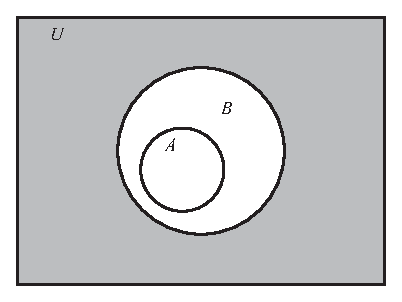
\includegraphics{figps-asubsetb2.eps}
\caption{Venn Diagram with $A \subseteq B$} \label{fig:asubsetb2}
\end{center}
\end{figure}
From the Venn diagram, it appears that  $A \cap B^c  = \emptyset $.  This means that  $A$  and  $B^c$  are disjoint.
%
The preceding example suggests that the following proposition is true:
\begin{center}
If  $A \subseteq B$, then  $A \cap B^c  = \emptyset $.
\end{center}
If we would like to prove this proposition, a reasonable ``backward question'' is, ``How do we prove that a set $\left( \text{namely } A \cap B^c \right)$ is equal to the empty set?''

This question seems difficult to answer since how do we prove that a set is empty?   This is an instance where proving the contrapositive or using a proof by contradiction could be reasonable approaches.  To illustrate these methods, let us assume the proposition we are trying to prove is of the following form:
\begin{center}
If  $P$, then  $T = \emptyset $.
\end{center}
If we choose to prove the contrapositive or use a proof  by contradiction, we will assume that  
$T \ne \emptyset $.  These methods can be outlined as follows:
\begin{itemize}
\item The contrapositive of ``If  $P$, then  $T = \emptyset $'' is, ``If $T \ne \emptyset $, then $\mynot P$.''  So in this case, we would assume  $T \ne \emptyset $ and try to prove $\mynot P$.

\item Using a proof by contradiction, we would assume $P$ and assume that  $T \ne \emptyset$.  From these two assumptions, we would attempt to derive a contradiction.

\end{itemize}
One advantage of these methods is that when we assume that  $T \ne \emptyset $, then we know that there exists an element in the set  $T$.  We can then use that element in the rest of the proof.  We will prove one of the conditional statements for Proposition~\ref{P:subsetprop} by proving its contrapositive.  The proof of the other conditional statement associated with Proposition~\ref{P:subsetprop} is Exercise~(\ref{exer:subsetprop}).
%\hbreak
\begin{proposition} \label{P:subsetprop}
Let $A$  and  $B$  be subsets of some universal set.    Then $A \subseteq B$ if and only if 
$A \cap B^c  = \emptyset $.
\end{proposition}
%
\begin{myproof}
Let  $A$  and  $B$  be subsets of some universal set.  We will first prove that if  $A \subseteq B$, then  $A \cap B^c  = \emptyset $, by proving its contrapositive.  That is, we will prove
\begin{center}
If   $A \cap B^c  \ne \emptyset $, then  $A \not \subseteq B$.
\end{center}
So assume that  $A \cap B^c  \ne \emptyset $.  We will prove that  $A \not \subseteq B$ by proving that there must exist an element  $x$  such that  $x \in A$  and  $x \notin B$.

Since  $A \cap B^c  \ne \emptyset $, there exists an element  $x$  that is in  $A \cap B^c $.  This means that
\[
x \in A\text{  and  }x \in B^c. 
\]
Now, the fact that  $x \in B^c $ means that  $x \notin B$.  Hence, we can conclude that
\[
x \in A\text{  and  }x \notin B.
\]
This means that  $A \not \subseteq B$, and hence, we have proved that if $A \cap B^c  \ne \emptyset $, then  
$A \not \subseteq B$, and therefore, we have proved that if $A \subseteq B$, then  $A \cap B^c  = \emptyset$.

The proof that if $A \cap B^c = \emptyset$, then $A \subseteq B$ is Exercise~(\ref{exer:subsetprop}).
\end{myproof}
\hbreak


\begin{prog}[\textbf{Proving Two Sets Are Disjoint}] \label{prog:disjointsets} \hfill \\
It has been noted that it is often possible to prove that two sets are disjoint by using a proof by contradiction.  In this case, we assume that the two sets are not disjoint and hence, their intersection is not empty.  Use this method to prove that the following two sets are disjoint.
\[
A = \{ x \in \Z \mid \mod{x}{3}{12} \} \quad \text{and} \quad B = \{ y \in \Z \mid \mod{y}{2}{8} \}.
\]
\end{prog}
\hbreak


\subsection*{A Final Comment}
We have used the choose-an-element method
\index{choose-an-element method}%
 to prove Propositions~\ref{P:SissubsetT}, \ref{P:setdifference}, \linebreak 
and~\ref{P:subsetprop}.  Proofs involving sets that use this method are sometimes referred to as \textbf{element-chasing proofs.}
\index{element-chasing proof}%
\index{proof!element-chasing}%
  This name is used since the basic method is to choose an arbitrary element from one set and ``chase it'' until you prove it must be in another set.
\hbreak

\endinput


\endinput

\begin{itemize}
  \item Preview Activity 1.
  \item Combine Preview Activities 2 and 3.
  \item After Proposition 4.8, show that $S \ne T$ by showing $S \not \subseteq T$.
  \item Progress Check 4.12.
  \item Progress Check 4.9.
  \item For Proposition 4.11, use $A - \left( A \cap B^c \right) = A \cap B$.
  \item Possibly the current Prop. 4.11 as a Progress Check.  Or delay this to a theorem in the next section.
  \item Possible Activity or addition:  $A - ( B \cap C ) = (A - B) \cap (A - C)$.  The sets are not equal but the right side is a subset of the left side.
  \item Disjoint sets.  Change Proposition 4.14 to a biconditional (see Activity 4.17).  Do the converse as a Progress Check or an exercise.
  \item Using the Choose an Element Method in a Different Setting as an activity.
\end{itemize}


\subsection*{Using the Choose-an-Element Method in a Different Setting}
We have used the choose-an-element method
\index{choose-an-element method}%
 to prove Propositions~\ref{P:SissubsetT}, \ref{P:setdifference}, \linebreak
and~\ref{P:subsetprop}.  Proofs involving sets that use this method are sometimes referred to as \textbf{element-chasing proofs.}
\index{element-chasing proof}%
\index{proof!element-chasing}%
  This name is used since the basic method is to choose an arbitrary element from one set and ``chase it'' until you prove it must be in another set.

The choose-an-element method, however, is a general proof technique and can be used in settings other than set theory.  It is often used whenever we encounter a universal quantifier in a statement in the backward process.  Consider the following proposition.
\begin{proposition} \label{P:divlinearcomb}
Let a, b, and  t  be integers with $t \ne 0$.  If  t  divides  a  and  t  divides  b, then for all integers  x  and  y,  t  divides  (ax + by).
\end{proposition}
%
Notice that the conclusion of the conditional statement in this proposition involves the universal quantifier.  So in the backward process, we would have
\begin{list}{}
\item $Q$:	For all integers  $x$  and  $y$, $t$  divides  $ax + by$.
\end{list}
\vskip10pt
%
The ``elements'' in this sentence are the integers  $x$  and  $y$.  In this case, these integers have no ``given property.''  (They are just integers.)  The ``something that happens'' is that 
$t$  divides  $\left(ax + by\right)$.  
%Of course, this quantified sentence could be written as a conditional statement as follows:
%\begin{list}{}
%\item $Q$:	If  $x$  and  $y$  are integers, then  $t$  divides  $\left(ax + by\right)$.
%\end{list}
%\vskip10pt
%
This means that in the forward process, we can use the hypothesis of the proposition and choose integers  $x$  and  $y$.  That is, in the forward process, we could have
\begin{list}{}
\item $P$:	$a$, $b$, and  $t$  are integers with $t \ne 0$, $t$  divides  $a$  and  $t$  divides  $b$.
\item $P1$:	Let  $x \in \Z$ and let  $y \in \Z$.
\end{list}
\vskip10pt
%
\noindent
The proof of this proposition is part of Activity~\ref{A:divlincomb}.
\hbreak

\begin{activity}[Exploring and Proving Proposition~\ref{P:divlinearcomb}] \label{A:divlincomb} \hfill
\begin{enumerate}
\item Whenever we encounter a new proposition, it is a good idea to explore the proposition by looking at specific examples.  For example, let  \linebreak
$a = 20$, $b = 12$, and  $t = 4$.  In this case,  $t \mid a$  and  $t \mid b$.  In each of the following cases, determine the value of  $\left(ax + by\right)$ and determine if $t$ divides 
$\left(ax + by\right)$.  \label{A:divlincomb1}

\begin{multicols}{3}
\begin{enumerate}
\item $x=1, y=1$
\item $x=1, y=-1$
\item $x=2, y=2$
\item $x=2, y=-3$
\item $x=-2, y=3$
\item $x=-2, y=-5$
\end{enumerate}
\end{multicols}

\item Repeat Part~(\ref{A:divlincomb1}) with  $a = 21$, $b =  - 6$, and  $t = 3$.

\item We started the forward-backward process for the proof of Proposition~\ref{P:divlinearcomb} following the discussion of this proposition.  Complete the following proof of Proposition~\ref{P:divlinearcomb}.
%
\addtocounter{theorem}{-2}
\begin{proposition}
Let a, b, and  t  be integers with $t \ne 0$.  If  t  divides  a  and  t  divides  b, then for all integers  x  and  y,  t  divides  ax + by.
\end{proposition}
%
\begin{myproof}
Let $a$, $b$, and  $t$  be integers with $t \ne 0$, and assume that $t$  divides  $a$  and  $t$  divides  $b$.  We will prove that for all integers  $x$  and  $y$,  $t$  divides  
$\left(ax + by\right)$.

So let  $x \in \Z$ and let  $y \in \Z$.  Since  $t$  divides  $a$, there exists an integer  $m$  such that $ \ldots .$
\end{myproof}
\end{enumerate}
\end{activity}
\hbreak
\addtocounter{theorem}{1}

\begin{activity}[The Converse of Proposition~\ref{P:subsetprop}] \label{A:converseprop} \hfill \\
We will explore the converse of Proposition~\ref{P:subsetprop}.  This converse states:

\begin{list}{}
\item \emph{Let $A$ and $B$ be subsets of some universal set $U$\!.  If $A \cap B^c = \emptyset$, then $A \subseteq B$}.
\end{list}

\begin{enumerate}
\item Let $U = \Z$ and let $A = \left\{ x \in \Z \mid x \geq 8 \right\}$ and 
$T = \left\{ x \in \Z \mid x \leq 2 \right\}$.  We then see that $A \cap T = \emptyset$.  So if we let $B$ be the subset of $\Z$ such that $B^c = T$, we then have an example of two sets such that $A \cap B^c = \emptyset$.  In this case, is $A$ a subset of $B$?  Explain.

\item Give an example of two sets $A$ and $B$ that are subsets of $\R$ and for which 
$A \cap B^c = \emptyset$.  In this case, is $A$ a subset of $B$?  Explain.

\item Is the converse of Proposition~\ref{P:subsetprop} true or false?  Justify your conclusion.
\end{enumerate}
\end{activity}
\hbreak




\endinput
